\documentclass[10pt, landscape]{article}
\usepackage[scaled=0.92]{helvet}
\usepackage{calc}
\usepackage{multicol}
\usepackage{ifthen}
\usepackage[a4paper,margin=5mm,landscape]{geometry}
\usepackage{amsmath,amsthm,amsfonts,amssymb}
\usepackage{color,graphicx,overpic}
\usepackage{hyperref}
\usepackage{newtxtext} 
\usepackage{enumitem}
\usepackage{amssymb}
\usepackage[table]{xcolor}
\usepackage{vwcol}
\usepackage{tikz}
\usetikzlibrary{arrows.meta}
\usetikzlibrary{calc}
\usepackage{mathtools}
\usepackage{nicematrix}
\usepackage[T1]{fontenc} %%% <--- NOTE THIS
% for relations
\usepackage{cancel}
\usepackage{ mathrsfs }
\usepackage{listings}
\usepackage{background}
\setlist{nosep}

\usepackage{etoolbox}
\makeatletter
\preto{\@verbatim}{\topsep=0pt \partopsep=0pt }
\makeatother

\backgroundsetup{
scale=1,
color=black,
opacity=0.4,
angle=0,
contents={}
% {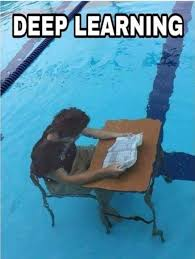
\includegraphics[width=\paperwidth,height=\paperheight]{image.png}}
}

\pdfinfo{
  /Title (CS2109S.pdf)
  /Creator (TeX)
  /Producer (pdfTeX 1.40.0)
  /Author (Seamus)
  /Subject (Example)
  /Keywords (pdflatex, latex,pdftex,tex)}

\lstset{language=Java,keywordstyle={\bfseries \color{black}}}

% Turn off header and footer
\pagestyle{empty}

\newenvironment{tightcenter}{%
  \setlength\topsep{0pt}
  \setlength\parskip{0pt}
  \begin{center}
}{%
  \end{center}
}

% redefine section commands to use less space
\makeatletter
% \renewcommand{\section}{\@startsection{section}{1}{0mm}%
%                                 {-1ex plus -.5ex minus -.2ex}%
%                                 {0.5ex plus .2ex}%x
%                                 {\normalfont\large\bfseries}}
% \renewcommand{\section}{\@startsection{section}{2}{0mm}%
%                                 {-1explus -.5ex minus -.2ex}%
%                                 {0.5ex plus .2ex}%
%                                 {\normalfont\normalsize\bfseries}}
% \renewcommand{\subsection}{\@startsection{subsection}{3}{0mm}%
%                                 {-1ex plus -.5ex minus -.2ex}%
%                                 {1ex plus .2ex}%
%                                 {\normalfont\small\bfseries}}%
% \renewcommand{\subsubsection}{\@startsection{subsubsection}{4}{0mm}%
%                                 {-1ex plus -.5ex minus -.2ex}%
%                                 {1ex plus .2ex}%
%                                 {\normalfont\small\bfseries}}%
\renewcommand{\section}{\@startsection{section}{1}{0mm}%
  {0.1ex} % space before
  {0.1ex} % space after
  {\normalfont\large\bfseries}}

\renewcommand{\subsection}{\@startsection{subsection}{2}{0mm}%
  {0.1ex} % space before
  {0.1ex} % space after
  {\normalfont\normalsize\bfseries}}

\renewcommand{\subsubsection}{\@startsection{subsubsection}{3}{0mm}%
  {0.1ex} % space before
  {0.1ex} % space after
  {\normalfont\small\bfseries}}
\renewcommand{\familydefault}{\sfdefault}
\renewcommand\rmdefault{\sfdefault}
% makes nested numbering (e.g. 1.1.1, 1.1.2, etc)
\renewcommand{\labelenumii}{\theenumii}
\renewcommand{\theenumii}{\theenumi.\arabic{enumii}.}
\renewcommand\labelitemii{•}
%  for logical not operator
\renewcommand{\lnot}{\mathord{\sim}}
\renewcommand{\bf}[1]{\textbf{#1}}
\newcommand{\abs}[1]{\vert #1 \vert}
\newcommand{\Mod}[1]{\ \mathrm{mod}\ #1}

\makeatother
\definecolor{myblue}{cmyk}{1,.72,0,.38}
\everymath\expandafter{\the\everymath \color{myblue}}
% Define BibTeX command
\def\BibTeX{{\rm B\kern-.05em{\sc i\kern-.025em b}\kern-.08em
    T\kern-.1667em\lower.7ex\hbox{E}\kern-.125emX}}
\let\iff\leftrightarrow
\let\Iff\Leftrightarrow
\let\then\rightarrow
\let\Then\Rightarrow

% Don't print section numbers
\setcounter{secnumdepth}{0}

\setlength{\parindent}{0pt}
\setlength{\parskip}{0pt}
%% this changes all items (enumerate and itemize)
\setlength{\leftmargini}{0.5cm}
\setlength{\leftmarginii}{0.5cm}
\setlist[itemize,1]{leftmargin=2mm,labelindent=1mm,labelsep=1mm}
\setlist[itemize,2]{leftmargin=4mm,labelindent=1mm,labelsep=1mm}

%My Environments
\newtheorem{example}[section]{Example}
% -----------------------------------------------------------------------

\begin{document}
\raggedright
\footnotesize
\begin{multicols*}{4}

% multicol parameters
% These lengths are set only within the two main columns
\setlength{\columnseprule}{0.25pt}
\setlength{\premulticols}{1pt}
\setlength{\postmulticols}{1pt}
\setlength{\multicolsep}{1pt}
\setlength{\columnsep}{2pt}

\begin{center}
    \fbox{%
        \parbox{0.8\linewidth}{\centering \textcolor{black}{
            {\Large\textbf{CS2109S}}
            \\ \normalsize{AY25/26 Sem 1}}
            \\ {\footnotesize \textcolor{myblue}{by ngmh}} 
        }%
    }
\end{center}
\vspace{-0.5em}

\section{Introduction}
\begin{itemize}
    \item PEAS: Performance Measure, Environment, Actuators, Sensors
    \item A rational agent chooses actions that maximise performance measure
    \item Agent percepts with sensors and perform actions with actuators
    \item Environments:
    \begin{itemize}
        \item Fully Observable (v/s Partially Observable): Agent's sensors give it access to complete state of environment, no need to keep track of state and no hidden information
        \item Single agent (v/s Multi agent): Presence of multiple agents in environment
        \item Deterministic (v/s Stochastic): Next state of environment is completely determined by current state and action executed by agent; if other rational agents actions matter it is also strategic, ignore uncertainty from actions of other agents even though agent cannot predict others actions
        \item Deterministic: Given a state and set of actions, we can precisely determine the next state
        \item Stochastic: Given a state and set of actions, we cannot determine the exact next state, but we know the probability of reaching each possible next state
        \item Episodic (v/s Sequential): Experience is divided into atomic episodes of agent perceiving then performing an action, and decision making is only dependent on the current episode; as opposed to current decision affecting future decisions
        \item Static (v/s Dynamic): Environment is unchanged while an agent is deliberating; semi-dynamic if environment does not change but agent's performance score does
        \item Discrete (v/s Continuous): Limited number of distinct, clearly defined percepts and actions
        \item Tic-Tac-Toe: Fully Observable, Deterministic, Strategic, Static, Sequential, Multi-agent
    \end{itemize}
\end{itemize}

\subsection{Intelligent Agents}
\begin{itemize}
    \item Agent program implements agent function that maps from percept histories to actions
    % \item Agent structures in increasing complexity:
    % \begin{itemize}
    %     \item Simple reflex agent: Choose action based on current world state
    %     \item Goal-based agent: Keeps track of state for decision making to reach goal
    %     \item Utility-based agent: Chooses action which maximises utility
    %     \item Learning agent: Critiques performance standard, changes decision making to learn
    %     \item Others: Model-based reflex agent, or combinations
    % \end{itemize}
    \item Exploitation v/s Exploration: Balance between learning more about world and maximising gain based on current knowledge
\end{itemize}

\subsection{Designing an Agent}
\begin{itemize}
    \item Search Problem: Goal is to find a state or path by exploring various possibilities
    \item Agent needs a goal, model of environment, and search algorithm
    \item Problem Formulation: States, Initial State, Goal / Test State, Actions, Transition Model, Action Cost Function
    \item Representation Invariant: Ensure that abstract states have corresponding concrete states with restrictions
    \item Every state has a set of actions, with branching factor $b$ if number of actions is less than or equal to $b$
    \item Transition Model: Uses transition function to produce next state given state and action
\end{itemize}

\section{Searching}
\begin{itemize}
    \item Path Cost: Cost of a path from any state to any state
    \item Optimal Path Cost: Cost of lowest cost path from any state to any state
    \item Complexity: Time (Number of nodes generated or expanded) or Space (Maximum number of nodes in memory)
    \item Completeness: Algorithm will find a solution for every problem instance (if one exists)
    \item Optimal: When an algorithm outputs a solution, it is guaranteed to be optimal (the best possible)
\end{itemize}

\section{Uninformed Search}

\subsection{BFS}
\begin{itemize}
    \item Maintain a frontier queue, and repeatedly expand shallowest unexpanded node
    \item Time and Space Complexity: Exponential wrt depth of optimal solution
    \item Complete if graph is finite
    \item Optimal if step cost is same everywhere
\end{itemize}

\subsection{Uniform Cost Search}
\begin{itemize}
    \item BFS but with non-identical edge weights
    \item Use a priority queue with path cost instead
    \item Time and Space Complexity: Exponential wrt tier of optimal solution
    \item Complete if $>0$ step cost everywhere and finite total cost
    \item Optimal if $>0$ step cost everywhere
\end{itemize}

\subsection{DFS}
\begin{itemize}
    \item Use a stack to maintain nodes, expand deeper nodes first
    \item Time Complexity: Exponential wrt max depth of tree
    \item Space Complexity: Polynomial wrt max depth of tree
    \item Not Complete when depth of search tree is infinite
    \item Not Optimal when solution is at shallower depth
    \item Complete with visited memory
\end{itemize}

\section{Informed Search}
\begin{itemize}
    \item Has information on search e.g. how good a state is
    \item Heuristic: Estimate of optimal path cost from any state to the goal state, e.g. straight line distance or Manhattan distance
    \item Best First Search: Use a priority queue, and evaluate in order of evaluation function of a state
    \item A* Search: Evaluation function $f(n)=g(n)+h(n)$, where $g$ is the cost to reach node $n$, and $h$ is the estimated cost from $n$ to goal
    \item Time and Space Complexity: Exponential
    \item Complete if edge costs are positive and branching factor is finite
    \item Optimality depends on heuristic
    \item Admissible Heuristic: For every node, $h(n) \leq h^*(n)$, where $h^*(n)$ is the optimal path cost to the goal state from $n$; heuristic never overestimates cost to reach goal
    \item Theorem: If $h(n)$ is admissible, A* without visited memory is optimal
    \item Consistent Heuristic: For every node, every successor $n'$ generated by action $a$ satisfies $h(n) \leq c(n,a,n')+h(n')$, $h(G)=0$, essentially triangle inequality
    \item Consistency implies Admissibility
    \item Theorem: If $h(n)$ is consistent, A* with visited memory is optimal
    \item Relaxed Problem: Has fewer restrictions, optimal solution to relaxed problem is an admissible heuristic
    \item If $h_1(n) \geq h_2(n)$ for all nodes, then $h_1$ dominates $h_2$, and is better for search if admissible
\end{itemize}

\subsection{Search Strategies}
\begin{itemize}
    \item Some search algorithms might not terminate without visited memory
    \item Can set a strict limit on resources an algorithm can use
    \item Gives rise to a search with polynomial memory which is complete and optimal
    \item Depth Limited Search: Limit search depth, backtrack when limit is hit
    \item Time Complexity: Exponential wrt depth limit
    \item Space Complexity: Polynomial wrt depth limit if used with DFS
    \item Not complete, not optimal (if used with DFS)
    \item Iterative Deepening Search: Search with increasing depth limits, returning a solution if found
    \item Time Complexity: Exponential wrt depth of optimal solution
    \item Space Complexity: Polynomial if used with DFS
    \item Complete, optimal (if step cost is same everywhere)
\end{itemize}

\subsection{Local Search}
\begin{itemize}
    \item Traverse state space by considering only locally-reachable states, repeatedly moving to better ones
    \item Typically incomplete and suboptimal
    \item Any-time property: Longer runtimes often have better solutions
    \item States represent potential solutions which might not be actual states
    \item Goal Test checks if a current state is the desired solution
    \item Successor Function generates neighboring states by modifying the current state
    \item Evaluation Function: Mathematical function used to assess the quality or desirability of a state which we either want to minimise or maximise
    \item Hill Climbing: Repeatedly move to the best successor based on eval until the current state is the best
    \item Shoulder: Objective function is flat and hard to move past
\end{itemize}

\subsection{Adversarial Search}
\begin{itemize}
    \item Multi-agent problems involve multiple agents which could be either cooperative or competitive
    \item Adversarial Games: Agents compete against each other; Zero-Sum: One player's gain is the other player's loss
    \item Turn-Taking Games: Next state of environment also depends on action of strategic opponents
    \item Game Tree represents all possible states and moves, and outcome is displayed below each terminal node
    \item Utility Function: Outputs value of a state from the perspective of our agent, which wants to maximise it
    \item Utility of non-terminal states is typically not known in advance and must be computed
\end{itemize}

\subsubsection{Minimax}
\begin{itemize}
    \item Assumes all players play optimally
    \item Player A: max, Player B: min
    \item Time Complexity: Exponential wrt maximum depth
    \item Space Complexity: Polynomial
    \item Complete if tree is finite
    \item Optimal if against optimal opponent
    \item Theorem: Minimax computes the optimal strategy for both players assuming both play optimally
    \item Theorem: If the opponent deviates from optimal play, the utility obtained by Player A is never less than the utility they would obtain against an optimal opponent
    \item Minimax explores the entire game tree in a depth first manner which can be costly
\end{itemize}

\subsection{Alpha Beta Pruning}
\begin{itemize}
    \item A variant of minimax which decreases the number of nodes that need to be evaluated
    \item $\alpha$: Highest value for A so far
    \item $\beta$: Lowest value for A so far
    \item On Player B's turn, if an action leads to a worse outcome, then the rest of the actions are irrelevant since the node will have at most that outcome which Player A does not want
    \item On Player A's turn, if an action leads to a better outcome, then the rest of the actions are irrelevant since the node will have at least that outcome which Player B is not interested in
    \item Initialise $\alpha=-\infty, \beta=+\infty$
    \item At a max node, set $v$ to be $max(v, v_i)$. Then set $\alpha=max(\alpha, v)$. If $v \geq \beta$, prune remaining nodes.
    \item At a min node, set $v$ to be $min(v, v_i)$. Then set $\beta = min(\beta, v)$. If $v \leq \alpha$, prune remaining nodes.
    \item $\alpha, \beta$ are not returned by reference!
    \item Theorem: Alpha-Beta pruning does not alter the minimax value and optimal move computed; it only reduces number of nodes evaluated
    \item Theorem: With good move ordering, runs in $O(b^{\frac{m}{2}})$
    \item Cutoff: Apply a strategy to halt search in middle due to computational constraints
    \item Estimate value of mid-game states with evaluation function which assigns a score to a game state
    \item A heuristic function estimates utility of a state, which should fall somewhere between the minimum and maximum possible utility for any state
    \item Derived from relaxed game, expert knowledge, or learnt from data
    \item Theorem: In a finite two-player, zero-sum game, minimax with cutoff and an evaluation function returns a move that is optimal with respect to the evaluation function at the cutoff (but not necessarily the true value)
\end{itemize}

\begin{verbatim}
def max_value(state, a, b):
    v = -INF // +INF
    for next_state in expand(state):
        v = max(v, min_value(next_state, a, b))
        // min(max)
        a = max(a, v) // b = min(b, v)
        if v >= b: return v // if v <= a:
return v
\end{verbatim}

\section{Machine Learning and Decision Trees}

\subsection{Machine Learning}
\begin{itemize}
    \item Some problems are intractable: They do not have an efficient solution for all cases
    \item Other problems are difficult because formulating the rules in a way that computers can process is hard
    \item A learning agent learns a function to identify patterns in the data and make decisions rather than explicitly solving it
    \item Machine Learning is a subfield of AI where computers learn without being explicitly programmed
    \item Supervised: Learn from labeled data (input-output pairs) to find a mapping from inputs to outputs
    \item Unsupervised: Learn from unlabeled data (input only) to find patterns or structure
    \item There is also semi-supervised or reinforcement learning
\end{itemize}

\subsection{Supervised Learning}
\begin{itemize}
    \item Data: Set of input-output (ground truth) pairs
    \item Model: Function that predicts output using input features
    \item Loss: Function used to assess model's performance
    \item Learning algorithm seeks to minimise loss of a model over a training dataset
    \item Model is evaluated on a test set using performance measures to estimate the generalisation of the model
    \item Classification: Predict a discrete label based on input features; output is a categorical value
    \item Regression: Predict a continuous numerical value based on input features; output is a real number
    \item A model or hypothesis refers to a function that maps from inputs to outputs and can be learned by a learning algorithm
    \item Performance measure is a metric evaluating how well the model performs
    \item A loss function quantifies the difference between the model's predictions and true outputs
    \item Examples of performance measures include mean squared error or mean absolute error for regression, and accuracy for classification
    \item For binary classification, we can look at the confusion matrix for true/false positives/negatives: "The prediction is [+/-] and it is [T/F]"
    \item $Accuracy=\frac{TP+TN}{TP+FN+FP+TN}$
    \item $Precision=\frac{TP}{TP+FP}$ if false positives are costly
    \item $Recall=\frac{TP}{TP+FN}$ if false negatives are costly
    \item $F1=\frac{2}{1/P+1/R}$
    \item A learning algorithm takes a training set of input-output pairs and finds a model which approximates the true relationship between inputs and outputs
\end{itemize}

\subsection{Decision Trees}
\begin{itemize}
    \item We are given a set of data points consisting of features and a target variable which are categorical
    \item A decision tree takes in an input vector of categorical attributes and outputs a predicted category
    \item Internal nodes represent tests on features, Branches correspond to outcomes of tests, Leaf nodes assign predictions
    \item A decision is made by checking the attribute value at each node and following it to the leaf node
    \item Prefer more compact decision trees, although they are less likely to be consistent with training data by chance
    \item Finding the optimal decision tree is NP-Hard, but it can be made tractable by greedy heuristics
    \item At each step, choose the feature that yields the greatest immediate information gain
    \item Entropy: Measure of uncertainty or randomness in a set of data, or number of bits used to represent it
    \item Entropy: $H(P(v_1),...P(v_n))=-\sum_{i=1}^nP(v_i)log_2P(v_i)$
    \item Common Entropies: $H(1)=0, H(1/2, 1/2)=1, H(1/3, 2/3)=0.918, H(3/5, 2/5)=0.971$
    \item For binary outcomes, $H(\frac{p}{p+n},\frac{n}{p+n})=-\frac{p}{p+n}log_2\frac{p}{p+n}-\frac{n}{p+n}log_2\frac{n}{p+n}$
    \item Specific Conditional Entropy: $H(Y|X=x)$ is the entropy of $Y$ conditioned that $X=x$, defined as $H(Y|X=x)=H(P(y_1 | x),...,P(y_k|x))$, only looking at a subset of samples fulfilling a condition
    \item Conditional Entropy: $H(Y|X)$ is the entropy of $Y$ when the value of $X$ is known, defined as $H(Y|X)=\sum_{x \in X}P(X=x)H(Y|X=x)$
    \item Information Gain: Measure of reduction in uncertainty after knowing the value of a specific variable, defined as $IG(Y;X)=H(Y)-H(Y|X)$
    \item Choose attributes with the highest information gain
    \item Stop splitting when all rows have same classification or there are no more attributes
    \item Theorem (Representational Completeness): For any finite set of consistent examples with discrete features and a finite set of label classes, there exists a decision tree that is consistent with the examples
    \item However, noise or outliers might cause learned decision tree to be unnecessarily complex or overfitting
    \item Pruning can produce simpler trees e.g. Max depth, Min Sample Leaves
    \item Max Depth: Limits maximum depth / length of longest path from a root node to a leaf node
    \item Min Sample Leaves: Set a minimum threshold for the number of samples required to be in a leaf node
    \item Partition continuous valued attributes into discrete intervals
    \item For missing values, come up with a way to populate them e.g. most common value of attribute, or same thing but only those with same output etc.
\end{itemize}

\section{Linear Regression}
\begin{itemize}
    \item Suppose each data point consists of features and a target variable, all of which are real numbers
    \item Given another data point without a target, we want to find a function that can predict a target for this new data point
    \item Linear Model: $h_w(x)=w_0x_0+w_1x_1+...+w_dx_d$ where $w_i$ are weights and $x_0=1$ is a dummy variable
    \item $h_w(x)=w^Tx=\sum_{j=0}^dw_jx_j$
    \item We want the linear model with the lowest loss on data, with a common measure being MSE
    \item MSE: $J_{MSE}(w)=\frac{1}{2n}\sum_{i=1}^n(h_w(x^{(i)})-y^{(i)})^2$, $\frac{\partial J_{MSE}(w)}{\partial w_j}=\frac{1}{n}\sum_{i=1}^n(h_w(x^{(i)})-y^{(i)})x_j^{(i)}$
    \item The gradient of $h$ is $\triangledown h(w)=[\frac{\delta h(w)}{\delta w_1}...\frac{\delta h(w)}{\delta w_d}]^T=[x_1...x_d]^T$
    \item To minimise a function $f(w)$, we find the point where $\triangledown f(w) = 0$, so for our multidimensional function, we want $\frac{\delta f(w)}{\delta w_i}=0$ for all $w_i$
    \item Minimum loss: $\triangledown J_{MSE}(w)=0$
    \item Normal Equation: Use $w=(X^TX)^{-1}X^TY$, derived from $X^T(Xw-Y)=0$
    \item However, the cost is $O(d^3)$ for inversion, and requires $X^TX$ to be invertible (not possible if features > data points)
    \item Gradient Descent: Start at a random $w$, and update $w$ with a step in opposite direction of gradient repeatedly until some termination criterion is satisfied
    \item $w_j=w_j-\gamma\frac{\delta J(w_0,...)}{\delta w_j}$ where $\gamma>0$ is the learning rate
    \item Convexity: For a line segment connecting any two distinct points on the graph, the line lies on or above the graph between two points
    \item Theorem: The MSE loss function is convex
    \item Linearly Dependent Features: A feature which can be expressed as a linear combination of other features
    \item Theorem: If the features in the training data are linearly independent, the function is strictly convex
    \item Theorem: For a linear regression model with MSE, gradient descent will converge to a global minimum provided the learning rate is chosen appropriately, which is unique if the features are linearly independent
    \item Learning Rate Scheduler: Decrease learning rate during training
    \item Larger features have greater updates to weights, so we need to scale them
    \item Min-max Scaling: $x_i'=\frac{x_i-min(x_i)}{max(x_i)-min(x_i)}$
    \item Standardisation: $x_i'=\frac{x_i-\mu_i}{\sigma_i}$, using normal distribution
    \item Alternatively have different learning rate for each weight
    \item Gradient descent can be very slow since it requires the entire dataset; can get stuck at local minimum or plateau on non-convex optimisation
    \item Batch Gradient Descent: Consider all training examples
    \item Mini-Batch Gradient Descent: Consider a subset of training examples at a time, cheaper per iteration, noisy gradient can help escape local minima
    \item Stochastic Gradient Descent: Select a random training example at a time
    \item $n$ points, needs maximum degree of $n-1$
\end{itemize}

\subsection{Feature Transformation}
\begin{itemize}
    \item Transform $d$ dimensional feature into $M$ dimensional, usually $M \geq d$ using a function e.g. polynomial, log, exp
    \item Theorem: The convexity of linear regression with MSE is preserved with feature transformation
    \item Model is usually $\hat{h}(x)=h(\phi(x))$, where $\phi$ is the feature transformation function and $h$ is the predictor
\end{itemize}

\section{Logistic Regression}
\begin{itemize}
    \item Given a set of data points with features and a target variable, but this time they are described by real numbers, and the target is either a positive or negative class (1 or 0)
    \item This is a classification problem (binary in this case)
    \item Sigmoid Function: $\sigma(x)=\frac{1}{1+e^{-x}}$, which is differentiable with derivative $\sigma'(x)=\sigma(x)(1-\sigma(x))$
    \item Logistic Model: Function of the form $h_w(x)=\sigma(w_0x_0+...+w_dx_d)=\sigma(w^Tx)$ where $x_0=1$ is a dummy variable
    \item The model's output is the probability of an input to be class 1, giving the confidence score of the model
    \item $\frac{\partial J_{BCE}(w)}{\partial w_j}=(h_w(x)-y)x_j$
    \item Example: Outputs $h_w(x)=P(Fail | x)=0.8$ means it predicts the probability of failure to be $0.8$
    \item To decide which class an input belongs to, compare the probability output with a given threshold
    \item Decision Boundary: Surface that separates different classes in the feature space, which is intersection between model's function and decision threshold, $(w_i-w_j)^Tx=0$
    \item Theorem: MSE is non-convex for logistic regression
    \item Cross-Entropy: Measures difference between two probability distributions over same set of outcomes, suppose $P$ is the true probability distribution and $Q$ is our model, then we have $H(P,Q)=-\sum_xP(x)log\ Q(x)$
    \item Binary Cross Entropy: Special case where there are only two possible outcomes, so $H(P,Q)=-P(1)log\ Q(1) - P(0)log\ Q(0)$
    \item BCE Loss: $J_{BCE}(w)=\frac{1}{n}\sum_{i=1}^n BCE(y^{(i)}, h_w(x^{(i)}))$
    \item Theorem: The BCE loss function is convex
    \item Partial derivative equation does not have a closed form
    \item Theorem: For a logistic model with BCE, gradient descent is guaranteed to converge to a global minimum provided the learning rate is chosen appropriately
    \item Data is linearly separable when a single linear decision boundary separates the different classes
    \item When it is not, the decision boundary required needs to be non-linear or more complex, which can be done with feature transformation
    \item Theorem: The convexity of a logistic model with BCE is preserved with feature transformation
    \item Multi-Class Classification: Either one vs one or one vs rest
    \item One vs One: Classifier for every pair of classes, need $K(K-1)/2$ of them, class with most votes is selected
    \item One vs Rest: Treat all other classes as single combined class, need $K$ of them, classifier with highest probability determines the class
    \item Multi-Label Classification: Labels might not be mutually exclusive
    \item Binary Relevance: Train one binary classifier per label
    \item Classifier Chain: Feed predictions of previous labels as features for subsequent labels which can capture dependencies although dependent on order
    \item Label Powerset: Treat each unique set of labels as a single multiclass label
\end{itemize}

\subsection{Topics in Supervised learning}
\begin{itemize}
    \item Generalisation: Model's ability to perform on unseen data
    \item Dataset Quality: Data should be relevant and balanced, but might contain noise
    \item Having more data typically leads to better performance
    \item Model Complexity: Size and expressiveness of model functions; higher model complexity allows for more sophisticated modeling of relationships
    \item A simple model is good for a simple ground truth but bad for complex ground truth (high bias, underfitting), retraining often leads to same model (low variance)
    \item Complex model overfits with scarce data, while it can fit better when data is abundant (low bias), retraining can lead to vastly different models (high variance)
    \item High Complexity: Has high error on unseen data, which reduces and converges as data quantity exists
    \item Low Complexity: High error on both unseen and training data even as data quantity increases, but does not diverge as much
    \item As model complexity increases, error decreases on unseen then increases again followed by decreasing again due to overparameterisation
    \item Hyperparameters: Settings that control behaviour of training algorithm but are not learned e.g. learning rate, feature transformations
    \item Hyperparameter Tuning: Optimising hyperparameters of a machine learning model to improve its performance (using validation set for evaluation)
    \item Techniques: Grid search, Random search, Local search, Successive halving, Bayesian optimisation
\end{itemize}

\section{Regularisation}
\begin{itemize}
    \item Overfitting: Model is too complex for underlying ground truth because it learns training data too well; including noise and fluctuations
    \item Often associated with large-magnitude weights
    \item $L_p$-norm: $||w||_p=(\sum_{j=0}^d|w_j|^p)^\frac{1}{p}$
    \item Regularisation: Introduce constraints to a loss function to prevent model from becoming too complex
    \item Augment loss function with regulariser, $J_{reg}(w)=J(w)+\lambda R(w), \lambda \geq 0$
    \item Common ones are $L_1 (|w_j|), L_2 (w_j^2), L_\infty (max|w_j|)$
    \item Lasso Regression: Linear regression + $L_1$ norm, Ridge Regression: Linear regression + $L_2$ norm, Elastic Net: Linear Regression + $L_1$ + $L_2$ norm
    \item The objective is still to minimise the regularised loss, which is when the derivative is 0
    \item Normal Equation: $w=(X^TX+\lambda I)^{-1}X^TY$
    \item Theorem (Invertibility): For $n \times d$ $X$ and $d\times d$ $I$, for any $\lambda > 0$, $X^TX+\lambda I$ is invertible
    \item Theorem (Solution Uniqueness): For any $\lambda >0$, ridge regression has a unique closed form solution given by the normal equation above
    \item Theorem ($L_2$ induces weight shrinkage): For any $\lambda > 0$, the $L_2$ norm of the regularised weight vector is strictly smaller than the non-regularised weight vector assuming a non-zero solution
    \item Theorem ($L_1$ penalty): If a feature has non-zero weight, the $L_1$ regulariser will penalise the feature with a constant penalty of $\lambda$ in terms of gradient
    \item Theorem ($L_1$ induces sparsity): For a feature to be included, its contribution to reducing the MSE loss must be exactly equal to the regularisation penalty $\lambda$ in terms of gradient, it not its weight will be set to exactly zero rather than pay the penalty
\end{itemize}

\subsection{Kernel Method}
\begin{itemize}
    \item Problem: A linear model will have an extremely large number of weights with respect to the number of features
    \item Primal Formulation has ${k+d \choose k}$ terms
    \item Theorem: For a linear model with weight vector $w$, the best weight vector minimising loss can be expressed as $w=\sum_{j=1}^n a_jx^{(j)}$, linear combination of training input
    \item Representer Theorem: A more generalised version where prediction is of form $f(w^Tx)$
    \item Primal and Dual Formulation: $h_w(x)=w^Tx=\sum_{j=1}^na_jx^{(j)^T}x=h_a(x)$
    \item For the dual formulation, we minimise the loss over $a$ instead of $w$
    \item For primal formulation, number of weights is all terms of maximum degree, while for dual formulation, it is proportional to number of data points
    \item Dual formulation is $\sum_{j=1}^n a_j \langle x^{(j)}, x\rangle$ (inner product)
    \item Theorem: For any feature mapping $\phi$, there must exist a function $k_\phi(u,v)$ that computes $\langle\phi(u), \phi(v)\rangle$ for any $u,v$; this is the kernel
    \item With kernel, the dual formulation is $h_a^\phi(x)=\sum_{j=1}^n a_j k_\phi(x^{(j)}, x)$
    \item Kernel Trick: We do not have to expand $\phi(x)$, we can simply compute kernel between $x^{(j)}, x$
    \item Polynomial Degree $k$ Kernel: $k_{pk}(u, v)=\phi_{pk}(u)^T\phi_{pk}(v)=(u^Tv)^k$, feature map is polynomial combinations of features with degree $\leq k$
    \item Gaussian Kernel with variance $s^2$: $k_{RBF}(u, v)=e^{-\frac{||u-v||^2}{2s^2}}$, feature map is an infinite list of scaled powers of the input features
    \item Mercer's Theorem: For any valid kernel $k_\phi$, there must exist a vector space with a feature mapping $\phi$
\end{itemize}

\section{Support Vector Machines}
\begin{itemize}
    \item Classification problem, each data point has $d$ features which are real numbers and the output is $-1,1$ for a negative and positive class
    \item SVM Model: $h_w(x)=sign(w^Tx)$
    \item Zero-offset hyperplane: Normal vector $w$ containing all $u$ where $w^Tu=0$
    \item Prediction: Use $sign(w^Tx)$, tells us which side it lies on
    \item Distance to hyperplane: $\frac{|w^Tx|}{||w||}$, LOP
    \item Margin: Distance between hyperplane and closest training data points, $\frac{1}{||w||}$, we aim to maximise this
    \item Support Vectors: Training data points on margin boundaries
    \item Dual Formulation: $h_a^\phi(x)=sign(\sum_{i=1}^na_i k_\phi(x^{(i)},x))$
    \item Theorem: For linearly separable data, the optimal dual-formulation SVM has $a_i>0$ iff it lies exactly on the boundary (support vectors), and $a_i = 0$ if it is strictly outside the margin boundary
    \item Theorem: For linearly separable data with $r$ dimensions, the number of support vectors is at least $r+1$, in practice it is much less than the number of data points
    \item Due to sparsity (most coefficients are zeroed out), we only need to store support vectors and their corresponding $a_i$
    \item The SVM model is given by $h_a(x)=sign(\sum_{x^{(i)} \in S} a_i k(x^{(i)},x))$
    \item Hyperplane is $w^Tx+b=0$, $b=-w^Tx$, check sign
\end{itemize}

\section{Unsupervised Learning}
\begin{itemize}
    \item Data where we do not have ground truths
    \item Clustering: Identify clusters in data
    \item Dimensionality Reduction: Find a lower-dimensional representation of the data while retaining relevant information
\end{itemize}

\subsection{K-means Clustering}
\begin{itemize}
    \item Centroid: Average of a set of data points, $\mu_j=\frac{1}{n_j}\sum_{i=1}^{n_j}x^{(i)}$, defines a cluster
    \item Randomly initialise centroids, assign points to the nearest centroids, then repeatedly update centroid of each cluster until convergence
    \item Distortion: Average square distance of each sample to its assigned centroid, $\frac{1}{n}\sum_{i=}^n||x^{(i)}-\mu_c(i)||^2$
    \item Theorem: Each step never increases distortion
    \item Could get stuck in local minima, either rerun many times with random initialisation or choose initial centroids better e.g. maximising distance between them
    \item K-Mediods: Use actual data point as cluster center
    \item Elbow Method: Use $k$ on elbow of the loss against $k$ graph
\end{itemize}

\subsection{Dimensionality Reduction}
\begin{itemize}
    \item Curse of Dimensionality: The number of samples needed to learn a class increases exponentially with number of features, $n=O(2^d)$
    \item Orthonormal Basis: Set of normalised vectors such that every vector can be expressed as a unique linear combination of the vectors in the set
    \item SVD: Decompose into $A=U\Sigma V^T$
    \item Theorem: WLOG, $d > n$, $A$ is $d \times n$, then the factorisation above has $d \times d$ $U$ with $d$ orthonormal columns and rows, $d \times n$ $\Sigma$ which is diagonal with non-increasing singular values, and $n \times n$ $V$ with $n$ orthonormal columns and rows
    \item $U$ is the new orthonormal basis, $\Sigma$ is the importance matrix, while $V^T$ is the linear combination coefficients
    \item The $n$ singular values tells us the importance of the new basis vectors
    \item A data point is a linear combination of basis vectors in $u$
    \item We keep the $r$ most significant vectors in the basis
    \item $u^Tv=\sum_{j=1}^du_jv_j=z||v||$ gives the LOP of $u$ onto $v$ times the norm of $v$
    \item $\tilde{U}$ defines the $r$ dimensional subspace of the feature space, and for any feature vector $x$, $\tilde{U}^Tx$ gives the linear combination coefficients in the new subspace
    \item So we have $r \times n$ $Z=\tilde{U}^TX^T$ which projects the data points onto the new lower-dimensional basis
    \item Theorem: For a fixed $r$, $\tilde{U}\tilde{U}^T\approx I$ with approximation error dependent on $r$, so we can reconstruct the data with $\tilde{X}^T=\tilde{U}Z, \tilde{X}^T=\tilde{U}\tilde{U}^TX^T\approx X^T$
    \item Mean Centered Data:
    \begin{itemize}
        \item Compute mean feature vector over all samples, $\bar{x} = \frac{1}{n}\sum_{i=1}^n x^{(i)}$
        \item Compute mean centered data points, $\hat{x}^{(i)}=x^{(i)}-\bar{x}$
        \item Use the mean centered data matrix
    \end{itemize}
    \item Variance: Expectation of $(X-E[X])^2$
    \item Theorem: Given a mean centered data matrix $\hat{X}^T$, the values $\frac{\sigma_j^2}{n-1}$ are variances of the data in the basis defined by the vectors $u^{(j)}$
    \item Theorem: Choose the minimum $r$ so that $\frac{\sum_{i=1}^r \sigma_i^2}{\sum_{i=1}^n\sigma_i^2} \geq 0.99$, then using this $r$, the original and mean centered data points satisfy $\frac{\sum_{i=1}^n ||\hat{x}^{(i)}-\tilde{x}^{(i)}||^2}{\sum_{i=1}^n||\hat{x}^{(i)}||^2}\leq 0.01$ for distortion
    \item PCA is a statistical application of SVD, capturing components that maximise the statistical variation of the data using sample covariance matrix
    \item PCA works well for natural images which have structured patterns and redundancy
\end{itemize}

\section{Neural Networks}
\begin{itemize}
    \item Neuron: Computes weighted sum of input features and passes result through activation function, $z=\sum_{j=0}^dw_jx_j, \hat{y}=g(z)$
    \item Activation Functions
    \begin{itemize}
        \item Sigmoid: $g(z)=\sigma(z)=\frac{1}{1+e^{-z}}$
        \item Identity: $g(z)=z$
        \item Tanh: $g(z)=tanh(z)=\frac{e^z-e^{-z}}{e^z+e^{-z}}$
        \item Relu: $g(z)=max(0, z)$
        \item Leaky Relu: $g(z)=max(az, z)$
    \end{itemize}
    \item Neurons can work as a learnable feature transformation function to produce a new feature as output
    \item Hidden Layer: Any layer between input and output layers
    \item Both hidden and output layers are fully-connected where every neuron is connected to every feature or neuron in the previous layer
    \item Multi-Layer Neural Networks with only fully-connected layers can also be called Multi-layer perceptrons
    \item Forward Propagation: Process by which input data passes through a neural network to generate the output
    \item Single-Layer Neural Network: $\hat{y}=g(W^Tx)$, $W$'s rows are the inputs for each neuron, while the columns are number of layer's neurons / output variables
    \item For multi-layered, compose $g$ and $W^Tx$ repeatedly
    \item Universal Approximation Theorem: NN with at least one hidden layer and non-linear activation function can approximate any continuous function
\end{itemize}

\subsection{Tasks}
\begin{itemize}
    \item Binary classification: Features are real numbers, while target is 0 or 1 for negative or positive class
    \item The hidden layers learn feature transformation, and the output layer has 1 neuron with the sigmoid activation function
    \item Multi-class classification: The output target is now a label in $[1,C]$
    \item One-hot encoding: Represent categorical labels as vectors of numbers, using a vector with 1 for the class and 0 everywhere else
    \item The output now has $C$ neurons, using the softmax activation function,  and we pick the class with the highest $\hat{y}_i$
    \item Softmax: Probability of belonging to class $i$ is $g(z_i)=\frac{e^{z_i}}{\sum_{j=1}^Ce^{z_j}}\in [0,1]$ where $z_i$ is the weighted sum value computed in neuron $i$, output sums to 1
    \item Single-output regression: The target is a real number
    \item The output layer has 1 neuron with the activation function being identity/none/sigmoid/tanh/...
    \item Multi-output regression: The target is a vector with $K$ real numbers
    \item Similar, but the output layer has $K$ neurons now
\end{itemize}

\subsection{Backpropagation}
\begin{itemize}
    \item Gradient Computation:
    \begin{itemize}
        \item Generate predicted value $\hat{y}$ for a given $(x,y)$ with $\hat{y}=g(\sum_{j=0}^dw_jx_j)$
        \item Compute the loss e.g. MSE: $L=\frac{1}{2}(\hat{y}-y)^2$
        \item Let $z=\sum_{j=0}^dw_jx_j, \hat{y}=g(z)$, the gradient of loss function is $\frac{\partial L}{\partial a}=(\hat{y}-y)(g'(z))(w_j)$, multiply with gradient or weight as we go along, sum if needed
    \end{itemize}
    \item Reversal:
    \begin{itemize}
        \item Compute gradient of loss wrt to $\hat{y}$
        \item Convert $g(z)$ to $g'(z)$ and treat $g'(z)$ as the weight associated with the corresponding edge
        \item Reverse the graph and compute gradients
    \end{itemize}
\end{itemize}

\section{Convolutional Neural Networks}
\begin{itemize}
    \item Images are represented as a grid of pixels
    \item Grayscale has one channel, while RGB has 3
    \item Large number of parameters, reduce using convolution
    \item Kernel / Filter: Matrix of weights
    \item Overlay the kernel, compute weighted sum using it, then slide and repeat to get output feature map
    \item Stride: Step size between positions
    \item Padding: Putting extra pixels around border of input data
    \item $H=\lfloor\frac{size - window\ size + 2\cdot padding}{stride} \rfloor + 1$
    \item Receptive Field: Region of input image that a particular neuron in the network is influenced by
    \item $r_i=r_{i-1}+(kernel_i-1) \times j_{i-1}$, $j_i = j_{i-1} \times stride_i$, $r_0=j_0=1$
    \item For multiple input channels use multidimensional kernel
    \item Multiple kernels give multidimensional feature map
    \item Convolutional Layer: Use convolution to extract features, then apply activation function
    \item Pooling Layer: Downsamples feature maps e.g. Max-Pool or Average Pool
    \item Cross-Entropy Loss: Between predicted output after softmax and one-hot encoded target, $CE(y^{(i)}, \hat{y}^{(i)})=-\sum_{j=1}^Cy_j^{(i)}log(\hat{y}_j^{(i)})$
\end{itemize}

\section{Recurrent Neural Networks}
\begin{itemize}
    \item Given data points consisting of a sentence and a target label for each word, predict whether each word is a verb
    \item One-hot encoding: Each vector has length similar to vocabulary size, 1 is position of respective word
    \item One-hot takes a lot of space, does not have semantic similarity, poor generalisation
    \item Input is one-hot encoding, while output is the predicted label for each word
    \item Need contextual information, cannot predict each label independently
    \item Hidden State: Memory storing information from the past, used to make prediction for the next input
    \item Time Step: Single iteration in RNN where it processes one element of a sequence
    \item $h^{[1]}=g^{[h]}((W^{[xh]})^Tx^{[1]}+(W^{[hh]})^Th^{[0]})$, $\hat{y}^{[1]}=g^{[y]}((W^{[hy]})^Th^{[1]})$ performs an update using the current data point and the hidden state
    \item Many-To-Many RNN: Takes in a sequence of inputs to produce a sequence of outputs
    \item Each hidden state is used as input to the next RNN layer together with encoded input at that position
    \item Each RNN layer produces this hidden state to be used
    \item Hidden state is fed into FC layer to produce output
    \item Deep Recurrent Neural Networks: Multiple RNN Layers between input and FC layer, each layer has hidden state similar to above, higher layers can learn more general abstractions
    \item Sentiment Analysis: Classify a sentence into negative or positive (0 or 1)
    \item Many-To-One: Many RNN layers each taking the hidden state output from the previous, only last one connects to FC layer and output
    \item Image Captioning: Given feature vector of an image, generate a descriptive sentence in one-hot encoding
    \item One-To-Many: Similar to Many-To-Many, but each RNN after the first uses the previous FC layer output as input rather than the encoded input vector
    \item Question Answering: Provide answer to a question, input and output are one-hot encoded, length might be different
    \item Many-To-Many, but first few RNN layers do not use output as input, use encoded input instead, last few RNN layers have output and use previous output as input
    \item Issues: Overfitting, Gradient Vanishing or Exploding
    \item Early Stopping: Halt training when models performance on validation set begins to worsen
    \item Dropout: Make neural network less reliant on specific neurons, randomly set some neurons' output to 0
    \item Vanishing Gradient: Small gradients get zeroed out due to repeated multiplication, change activation function to solve
    \item Exploding Gradient: Large gradients get multiplied until they overflow, use gradient clipping to bound range
\end{itemize}

\section{Attention}
\begin{itemize}
    \item For RNN, information from beginning of sequence must travel through long intermediate steps and might be degraded when it reaches the end
    \item Attention: Allows NN to selectively focus on relevant parts of its input data when producing an output
    \item Model like YouTube search
    \item Query: Represents what current position is trying to retrieve (Search Query)
    \item Key: Describe what each position offers in terms of information (Video Keyword)
    \item Value: Actual information retrieved when position is attended to (Video Content)
    \item Query is compared to all keys to determine relevance
    \item Relevance / attention score is used to retrieve weighted sum of all values; the relevant context
    \item Self-Attention Layer: Each input element can find relevant context from all elements in the same sequence
    \item Computation:
    \begin{enumerate}
        \item Transform inputs into QKV using learnable matrices; $q^{[t]}=W^qx^{[t]}$, $k^{[t]}=W^kx^{[t]}$, $v^{[t]}=W^vx^{[t]}$, $d_q=d_k$, $x^{[t]}\in \mathbb{R}^d$
        \item Compute attention scores with Softmax; $a_{i1}=\frac{(k^{[i]})^Tq^{[1]}}{\sqrt{d_k}}$, $k^{[t]} \in \mathbb{R}^{d_k}$, $a'_{i1}=\frac{e^{a_{i1}}}{\sum_{i=1}^Te^{a_{i1}}}$, $T$ is the length of the sequence; $a_{ij}$ is the amount that token $i$ attends to token $j$
        \item Dot products are scaled to prevent softmax from being pushed into regions where it has extremely small gradients
        \item Compute weighted sum of all values; $h^{[1]}=\sum_{i=1}^Ta'_{i1}v^{[i]}$, this forms the hidden state
        \item $Q/K/V = W^{Q/K/V} X$, $A = \frac{Q^TK}{\sqrt{d_k}}$, $A'=softmax(A)$, $H=VA$
    \end{enumerate}
    \item Masked Self-Attention Layer: Each input element can find relevant context from previous elements and current element itself, similar but $a_{ij}=-\infty$ if $i>j$, can only use those coming before current time step
    \item Cross-Attention Layer: Elements can find relevant context from another sequence, Key and Value use $z^{[t]}$ instead rather than $x^{[t]}$
\end{itemize}

\subsection{Attention Neural Networks}
\begin{itemize}
    \item Replace RNN layer with hidden state chains with self-attention layer now, producing hidden state for each encoded input
    \item Does not consider position of a word
    \item Positional Encoding: Inject positional information into original input vectors, $x'^{[t]}=x^{[t]}+PE^{[t]}$
    \item $PE^{[t]}$ must be unique for each position, consistent (not affected by length of sequence), and bounded
    \item Large $PE$ might drown out actual meaning
    \item Use $\sin$ or $\cos$ to generate kth element using $PE_k^{[t]}=\sin(\frac{t}{C^{\frac{k}{d}}})$ if $k\%2=0$, $\cos(\frac{t}{C^{\frac{k-1}{d}}})$ otherwise
    \item Attention NN: Many-to-Many: Inputs are positionally encoded, and BCE loss is taken on output
    \item ANN: Many-to-One: Uses CLS (Classification Token) vector prepended to sequence, used to capture summary information of the entire input sequence and minimise training loss, hidden state for it is used by FC layer to produce output
    \item ANN: One-to-Many: Begin vector added after encoded feature vector, should be added into vocabulary and encoded like other words, have masked self-attention layer between input and hidden state, so each input can find context from previous elements
    \item Teacher Forcing: Used for sequence prediction; input for next step is true target, not model's current prediction
    \item No waiting, all output can be generated simultaneously
    \item Not available during testing, can lead to train-test mismatch, can gradually reduce teacher forcing over time
    \item ANN: Many-to-Many: have encoder and self attention layer generating initial hidden states, then BEGIN token feeding into masked self attention layer
    \item Masked self attention layer feeds into hidden states which feed into cross attention layers into FC layer into output
    \item Outputs piped back into masked self-attention layer
    \item Encoder: Reads input sequence and compresses information into vectors
    \item Decoder: Takes context vectors from encoder and generates new output sequence element by element
\end{itemize}

\subsection{Transformer}
\begin{itemize}
    \item Deep attention neural network based on encoder and decoder building blocks
    \item Feed Forward Network: FC Layer, ReLU, FC Layer
    \item Encoder Block: Self-attention layer, Feed forward network
    \item Decoder Block: Masked self-attention layer, Cross-attention layer, Feed-forward Network
    \item Encoder: Stack of encoder blocks, Decoder: Stack of decoder blocks
    \item Generative Pretrained Transformers (GPT) are build on transformer architecture
\end{itemize}

\section{Unsupervised Learning with NN}

\subsection{Dimension Reduction}
\begin{itemize}
    \item Autoencoder: NN which learns to compress data, consisting of encoder and decoder
    \item Encoder: Takes high dimensional input data and generates compressed data
    \item Decoder: Takes compressed data and attempts to reconstruct the original high-dimensional input data
    \item Must learn to keep input's important features in compressed data
    \item Compression / Reconstruction: Use layers that progressively get smaller / larger
    \item Use MSE loss, reconstruction loss measures how different reconstructed output is form original input
\end{itemize}

\subsection{Model Pre-Training}
\begin{itemize}
    \item Given a set of images, classify them into subsets
    \item Train model exclusively on labeled subset, wastes unlabeled subset
    \item New task: Solvable using unlabeled input image, but challenging enough to force model to deeply understand input image, and yields useful learned understanding
    \item Rotation Prediction: Assign label based on which rotation is applied, trained on image and rotated image pairs
    \item If model is not aware of concepts in images, it would not be able to recognise rotation
    \item Train model on invented task, create neural network for image classification, train model with labeled subset
    \item Pre-training, for feature transformation, initialise with trained weights, prediction part is randomly initialised
    \item Contrastive Learning: Train model to contrast samples, pull feature vector of similar images together, push feature vector of dissimilar images apart so model can learn to distinguish objects
    \begin{enumerate}
        \item Take input, create different version of it to form positive pairs
        \item Use other images to form negative pairs
        \item Use CNN to extract feature vector for each image
        \item Train model so that high similarity has large value and low similarity has small value
        \item $p^{(i)}=sim(z^{(i)}, z'^{(i)})/\tau, exp(p^{(i)})$
        \item $n^{(ij)}=sim(z^{(i)}, z^{(j)})/\tau, exp(n^{(ij)})$
        \item $sim(u,v)=\frac{u^Tv}{||u||||v||}$, $-1 \leq sim(u,v) \leq 1$, $\tau$ is a constant scaling factor
        \item Minimise $\ell^{(i)}=-log(\frac{exp(p^{(i)})}{exp(p^{(i)})+exp(n^{(ij)})})$
        \item The pre-trained model weights can be used in image classifier model
    \end{enumerate}
    \item Image Inpainting: Cut out random patch from an image and mask it, then ask model to fill in missing patch, model needs to understand the content of the image, learned weights on encoder can be use for image classification model initialisation
    \item Unlabeled Text: Given sequence of text, model needs to predict next word, by understanding grammar and syntax
\end{itemize}

\end{multicols*}

\end{document}